\chapter{Proof of Concept}
\label{sec:proofofconcept}

% PHP/XEDUB installation: https://ubuntuforums.org/showthread.php?t=525257
%						  https://www.youtube.com/watch?v=OlcsQ8TCU3A
%	> sudo add-apt-repository ppa:ondrej/php
%	> sudo apt-get update
%	> sudo apt-get apache2
% 	> sudo apt-get install php7.1-dev php-pear php7.1-mbstring php7.1-cgi	  			// old... > sudo apt-get install php5-dev php-pear
%	> sudo apt-get install libapache2-mod-php7.0
% 	> sudo pecl install xdebug
% 	> find / -name 'xdebug.so' 2> /dev/null
% 	/usr/lib/php5/20060613/xdebug.so
% 	> sudo gedit /etc/php/7.1/apache2/php.ini		
%		[xdebug]
%		zend_extension=/usr/lib/php/20160303/xdebug.so
%		xdebug.default_enable=1
%		xdebug.idekey=PHPSTORM
%		xdebug.remote_enable=1
%		xdebug.remote_port=9000
%		xdebug.remote_connect_back=1

% Enabling error msg. Set "`display_errors = On"' in:
%	> sudo gedit /etc/php/7.1/apache2/php.ini	

% Change document root:
% 	> sudo gedit /etc/apache2/sites-available/000-default.conf
%	> sudo gedit /etc/apache2/apache2.conf
% 	> sudo /etc/init.d/apache2 restart

% Installing grunt (as npm package):
%	> npm init
%	> npm install grunt --save-dev
%	create Gruntfile and update package.json according to: https://gruntjs.com/getting-started and http://www.wearecube.ch/from-less-to-css-with-grunt-js/
%	> npm install
%	> grunt
%					// > grunt watch &				// grunt watch will be stoped when the commandline closes

% installing composer/twig:
% 	download to project root: https://getcomposer.org
% 	> php composer-setup.php --filename=composer
%	create composer.json in project root. content:
% 		{
%			"require": {
%   			"twig/twig": "1.*",
%			    "twbs/bootstrap": "3.3.7"
%  			}
%		}
%	> php composer.phar install 		or			php composer.phar update
%	> sudo chown www-data:www-data bookinganalyzerimpl/compilation_cache/

% https://nikic.github.io/2011/12/12/How-big-are-PHP-arrays-really-Hint-BIG.html
% installing redis
%	> sudo pecl install redis
%	Adding "extension=redis.so" to php.ini
%	  	> sudo gedit /etc/php/7.1/apache2/php.ini	
%	  	> sudo gedit /etc/php/7.1/cli/php.ini	
% 	> sudo /etc/init.d/apache2 restart
%
%	> wget http://download.redis.io/releases/redis-3.2.8.tar.gz
%	> tar xzf redis-3.2.8.tar.gz
%	> cd redis-3.2.8
%	> make
% 	> ~/programs/redis-3.2.8/src/redis-server
% http://www.codeforge.com/article/214557


% Getting bookinganalyzerimpl to run:
% git clone git@github.com:soultemptation/bookinganalyzerimpl.git
% npm install
% grunt
% php composer.phar install

% Remove duplicates:
%			Find duplicates:
%			> egrep -o '^[^@]+' u611a_10_normalized_geocoded.csv > text.csv 	// Get everything before first @
%			> sort text.csv > text_sorted.csv									// Sort it
%			> uniq -d text_sorted.csv > text2_duplicates.csv					// Remove duplicates
% 	> tac u611a_10_normalized_geocoded.csv | sort -k1,1 -r -u -t@ > text5.csv
%	> tac text5.csv > text6.csv
%	Move last line of text6.csv to the beginning

\section{Datenvorbereitung}
\label{sec:proofofconcept:datenvorbereitung}

% Feature selection
% https://en.wikipedia.org/wiki/Feature_selection
% http://dollar.biz.uiowa.edu/~street/research/dmoc.pdf
% http://www.jmlr.org/papers/volume3/guyon03a/guyon03a.pdf

Die Daten müssen für die Verwendung im Proof of Concept vorbereitet werden. Dazu wurden zwei Programme geschrieben um die Daten anzureichern. Die Datentransormationen wurden anschliessend gemäss \cref{sec:recherche:datenvorbereitung} mit dem Programm RapidMiner durchgeführt.

\subsection{Datenerweiterung}
\label{sec:proofofconcept:datenvorbereitung:datenerweiterung}
Die Programme für die Datenanreicherungen sind jeweils eine Kommandozeilen-Software welche hier vorgestellt werden.

\subsubsection{Land, Region, Ortschaft}
\label{sec:proofofconcept:datenvorbereitung:datenerweiterung:landregionortschaft}
Es wurde ein Programm für die Anreicherung vom Land, der Region sowie der Ortschaft der Objekte erstellt. Es erwartet eine \gls{csv} Datei mit einem @-Zeichen als Feldseparator, sowie das Feld "`NREF"' welches in jeder Zeile vorkommen muss und die ID des Objektes beinhaltet. Der Quellcode ist einsehbar in Github unter \url{https://github.com/soultemptation/bookinganalyzerdestinations}.

Die Software verarbeitet Zeile für Zeile der Datei und fügt am Ende drei Felder mit den Namen "`country"', "`region"' und "`place"' an. Um die Daten zu erhalten wird der Such-Service von Interhome angesprochen, welcher die drei Informationen zurückliefert. Als Parameter des Services wird die `NREF"' des Objektes übergeben. 

Es kann sein dass das Objekt bei Interhome nicht mehr vorhanden ist und der Service nichts zurück liefert. Deshalb gibt es nach der Ausführung des Programmes Buchungen welche keine Informationen für das Land, die Region und die Ortschaft besitzen.

Im Programm wird ein Cache verwendet, welcher für jede "`NREF"' das Land, die Region und die Ortschaft zwischenspeichert. Wenn eine "`NREF"' zum zweiten mal angefragt werden soll, können die Daten aus dem Cache bezogen werden und es muss kein weiterer Service Aufruf durchgeführt werden. Für die 133'001 Buchungen mussten dank des Caches nur 78'342 Anfragen an den Service gestellt werden.

\subsubsection{Geolocation}
\label{sec:proofofconcept:datenvorbereitung:datenerweiterung:geolocation}
Das Programm für die Anreicherung der Geolocation erwartet wie die im \cref{sec:proofofconcept:datenvorbereitung:datenerweiterung:landregionortschaft} vorgestellte Software eine \gls{csv} Datei, in welchem die Felder mit einem @-Zeichen getrennt sind, sowie die Attribute "`CUSTRAS"' (Strasse), "`CUCNTRY"' (Land), "`CUZIP"' (Postleitzahl) und "`CUORT"' (Ort). Unter \url{https://github.com/soultemptation/BookingAnalyzerGeocoding} ist der Quellcode abgelegt. 

Um die Adresse in Geo-Koordinaten umzuwandeln wurde die "`Locations API"' von Bing Maps (Microsoft) verwendet (siehe \url{https://msdn.microsoft.com/en-us/library/ff701715.aspx}). Da der Service nicht kostenlos ist und 133'001 Geocoding-Anfragen gesendet werden mussten, wurde eine Lizenz benötigt welche an einen "`API Key"' gebunden ist. Es konnte eine Studenten-Lizenz erworben werden, welcher 10'000 Anfragen pro Tag erlaubt.

Das Programm geht jede Zeile der Datenquelle durch und sendet eine Anfrage an die "`Locations API"'. Übergeben wird die Adresse des Kunden sowie ein "`API Key"' für die Authentifizierung. Die Anfrage ist folgendermassen aufgebaut:

\blockquote[]{http://dev.virtualearth.net/REST/v1/Locations?countryRegion=\textbf{\{Zweistelliger Ländercode\}}\&locality=\textbf{\{Stadt\}}\&postalCode=\textbf{\{Postleitzahl\}}\&addressLine=\textbf{\{Strasse und Hausnummer\}}\&includeNeighborhood=0\&maxResults=1\&key=\textbf{\{API Key\}}}

Um zum Beispiel die Geolocation der ZHAW Zürich anzufragen, kann folgender Request angesetzt werden:

\blockquote[]{http://dev.virtualearth.net/REST/v1/Locations?countryRegion=\textbf{CH}\&locality=\textbf{Zurich} \&postalCode=\textbf{8021}\&addressLine=\textbf{Lagerstrasse 41}\&includeNeighborhood=0\&max Results=1\&key=\{API Key\}}

Bing Maps liefert dafür die Koordinaten "`47.37766, 8.53259"' zurück. In der \cref{fig:proofofconcept:datenvorbereitung:datenerweiterung:geolocation:1} ist die Adresse auf einer Karte eingezeichnet.

\begin{figure}[H]
	\RawFloats
	\centering
	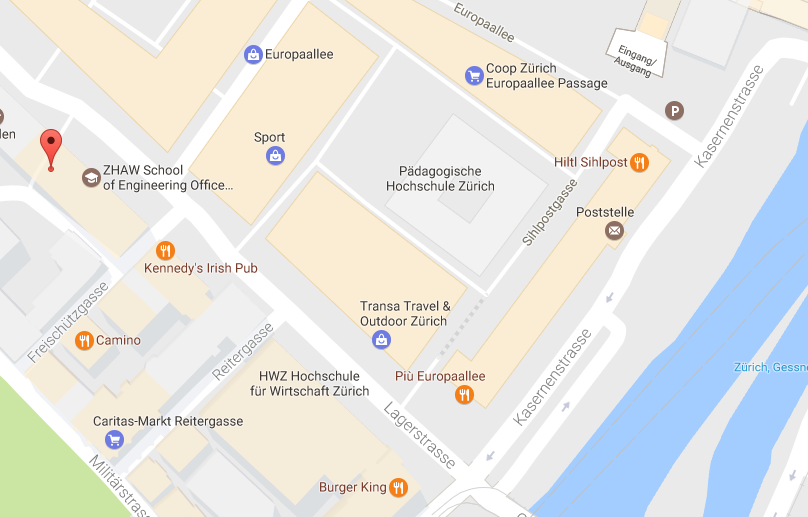
\includegraphics[width=1\textwidth]{images/bing-maps-result}
	\caption{Resultat des Geocodings von Bing Maps.}
	\label{fig:proofofconcept:datenvorbereitung:datenerweiterung:geolocation:1}
\end{figure}

\subsection{Datenvorbereitung mit RapidMiner}
Im \cref{sec:recherche:datenvorbereitung} wurde beschrieben, wie die Daten vorbereitet werden sollen. Dieser Abschnitt zeigt auf wie das Program RapidMiner verwendet wurde um diese Vorgaben zu erfüllen. \cref{fig:recherche:rapidminer:1} zeigt den definierte Prozess auf.

%Zuerst werden die Daten aus dem \gls{csv} File geladen. Anschliessend die Attribute gemäss \cref{fig:recherche:attributeinschraenkung:2} eingeschränkt sowie die Diskretisierung entsprechend \cref{fig:recherche:datenvorbereitung:1} und \ref{fig:recherche:datenvorbereitung:2} durchgeführt.

\begin{figure}[htb]
	\begin{subfigure}[t]{1\textwidth}
		\centering
		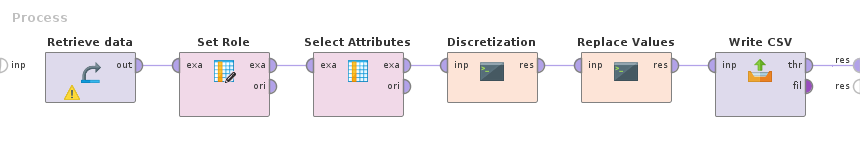
\includegraphics[width=1\textwidth]{images/rapidminer-process}
		\caption{Hauptprocess}
		\label{fig:recherche:rapidminer:1:1}
	\end{subfigure} \\
	\begin{subfigure}[t]{0.5\textwidth}
		\centering
		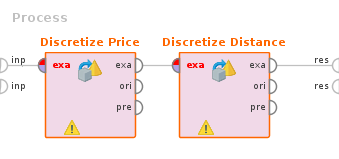
\includegraphics[width=1\textwidth]{images/rapidminer-process-discretization}
		\caption{Subprocess für die Diskretisierung}
		\label{fig:recherche:rapidminer:1:2}
	\end{subfigure}
	\begin{subfigure}[t]{0.8\textwidth}
		\centering
		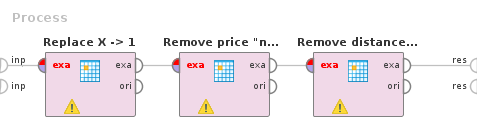
\includegraphics[width=1\textwidth]{images/rapidminer-process-replace-values}
		\caption{Subprocess für die Ersetzung von Attributwerten}
		\label{fig:recherche:rapidminer:1:3}
	\end{subfigure}
	\caption{RapidMiner Prozess für die Vorbereitung der Daten}
	\label{fig:recherche:rapidminer:1}
\end{figure}

%"`"'
 In \ref{fig:recherche:rapidminer:1} wird der Prozess gezeigt wie er im RapidMiner definiert wurde. Nachfolgend werden die einzelnen Schritte 
 \begin{itemize}
 	\item Retrieve data: Lädt die Buchungen aus der Datenquelle damit diese bearbeitet werden können. 
 	\item Filter Exapmles: \todo{Filter Example}.
 	\item Select Attribute: Entfernt alle Attribute welche nicht in der \cref{fig:recherche:attributeinschraenkung:2} aufgeführt werden.
 	\item Generate ID: Generiert eine ID für die eindeutige Identifikation der Buchungen.
 	\item Normalize: Normiert nummerische Werte auf einen Interval $0 \leq x \leq 1$ (siehe \cref{sec:recherche:datenvorbereitung:normierung} \nameref{sec:recherche:datenvorbereitung:normierung}).
 	\item Weeklyprice: Berechnet den Wochenpreis einer Buchung (siehe \cref{sec:recherche:datenvorbereitung:normierung} \nameref{sec:recherche:datenvorbereitung:normierung}).
 	\item Discretization: Ist ein Unterprozess welcher in \cref{fig:recherche:rapidminer:1:2} dargestellt ist.
	 	\begin{itemize}
	 		\item Discretize Price: Diskretiert die Preise gemäss \cref{fig:recherche:datenvorbereitung:2}. Die Preisspannen die nicht im Resultat verwendet werden sollen werden später im Schritt "`Replace Values"' entfernt.
	 		\item Discretize Distance: Diskretiert die Distanzen gemäss \cref{fig:recherche:datenvorbereitung:1}. Distanzspannen die nicht im Resultat verwendet werden sollen werden später im Schritt "`Replace Values"' entfernt.
	 	\end{itemize}
 	\item Replace Values: Ist ein Unterprozess welcher in \cref{fig:recherche:rapidminer:1:3} dargestellt ist.
 		\begin{itemize}
			\item Replace X -> 1 und Replace empty -> 0: Wandelt boolsche Werte in 1 und 0 um (siehe \cref{sec:recherche:datenvorbereitung:boolschewerte} \nameref{sec:recherche:datenvorbereitung:boolschewerte}). 
			\item Remove price ...: \todo{}
 		\end{itemize}
 	\item Remove Price: Entfernt den gesamt Preis der Buchung. Dieser muss beim Schritt "`Select Attribute"' hinzugefügt werden damit der Wochenpreis berechnet werden kann. Im Resultat wird das Attribut jedoch nicht mehr benötig.
 	\item Write CSV: Speichert das Resultat im \gls{csv} Format auf die Festplatte ab.
 \end{itemize}

\section{Kommunikationsablauf}
\label{sec:proofofconcept:kommunikationsablauf}
In \cref{fig:proofofconcept:kommunikationsablauf:1} wird der Kommunikationsablauf aufgezeigt, welcher zwischen dem Server und dem Browser des Benutzers stattfindet. Sobald der Benutzer eine Analyse startet wird eine Anfrage an den Server gestellt. Dieser erstellt einen Hintergrundprozess welcher die Analyse durchführt und gibt danach direkt eine Antwort an den User zurück. 

Der Hintergrundprozess führt die Analyse durch und schreibt periodisch einen Zwischenstand im \gls{HTML}-Format in eine Datei.

Sobald die Analyse vom Server angestossen wurde kann dieser eine Rückmeldung zum Benutzer senden mit der Nachricht, dass die Analyse gestartet wurde. Der Browser des User beginnt darauf hin, die \gls{HTML}-Datei auf dem Server nach dem Zwischenstand abzufragen bis die Analyse beendet ist.
\begin{figure}[H]
	\RawFloats
	\centering
	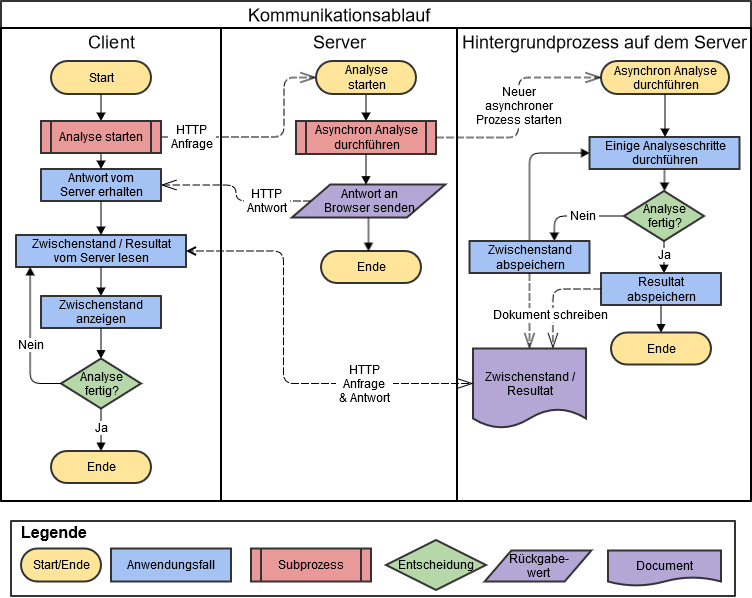
\includegraphics[width=1\textwidth]{images/communication-flow}
	\caption{Kommunikationsablauf}
	\label{fig:proofofconcept:kommunikationsablauf:1}
\end{figure}

Eine Webanfrage hat normalerweise eine obere Laufzeitgrenze von 30 Sekunden. Bis dann muss der Server eine Antwort liefern, sonst wird dem Benutzer eine Fehlermeldung angezeigt und der Prozess auf dem Server gestoppt. Da die Analyse, je nach Datenmenge, einige Minuten bis Stunden dauern kann musste dafür eine Lösung gefunden werden. Dank des Hintergrundprozesses kann der Server rasch eine Antwort liefern, der Browser dem Benutzer eine Meldung anzeigen und die Analyse länger als 30 Sekunden laufen.



